\appendix
\section{L1 Trigger Studies for the H plus zero and one jets final state}
\label{app:L10j}


\section{L1 Trigger Studies for the VBF final state}
\label{app:L1}

High rate issues will affect, during 2011 run, also the L1 electron trigger seeds. 
Single-object-based seeds, which require the presence of an ECAL tower with an energy readout higher than the chosen 
threshold, will become unavailable in low $E_T$ range (i.e. below $30 \ GeV$) so we developed a new L1 algorithm
based on the presence of both an high energy EM deposit and two hadronic deposits (AKA L1 Jets).\\

Again, as presented in section \ref{sec:trigger}, the design of the algorithm is driven by the complex topology of the final
states. In the case of the L1 we have a correspondance between the electron coming from the W and an highly energetic 
ECAL tower deposit and between the \textit{tagging} jets and the hadronic deposits, which therefore must have a 
significant pseudorapidity separation.\\

The cut optimization study on the EM deposit threshold and the hadronic deposit threshold has been done and results are 
shown in Fig. \ref{fig:EleL1_EGEt_JetEt} both for rate and efficiencies. L1 Jet (EM + Hadronic deposit) are cleaned from pure
EG objects, i.e. we are not considering those L1 Jets which are matched with L1 electrons (EM deposit).


\begin{figure}[htb]
  \begin{center}
    \includegraphics[width=0.45\textwidth]{plots/Trigger/L1_EGEtVsJetEt_Rate.png}
    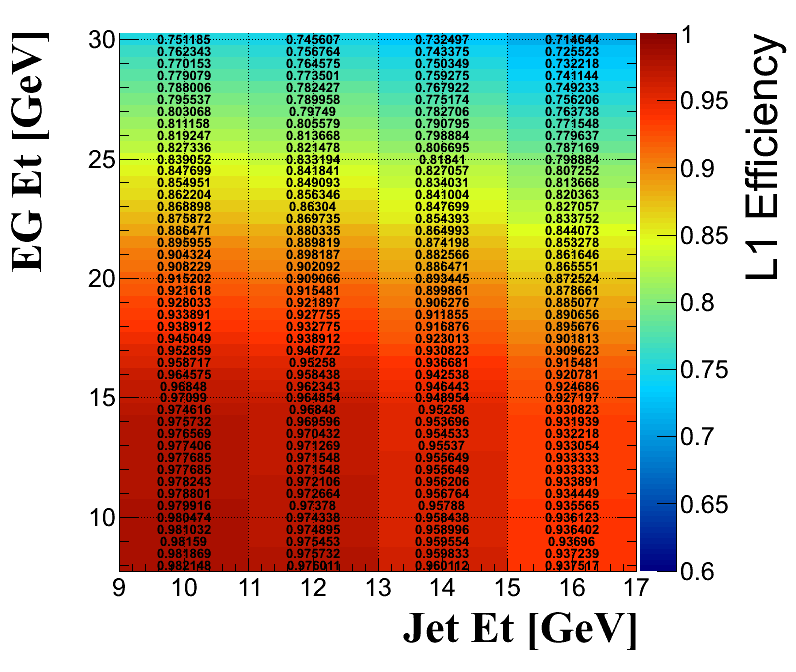
\includegraphics[width=0.45\textwidth]{plots/Trigger/HLT_EGEtVsJetEt_Eff.png}
    \caption{EGamma plus Di-Jet rate (left) and efficiencies (right) at L1. Rate projections are
             done for an instantaneous luminostity of  $\ 5 \cdot 10^{32}\ cm^{-2}s^{-1}$ while efficiencies
             are evaluated on a $H\rightarrow WW\rightarrow \ell \nu_{\ell} + qq'$ sample.  }
    \label{fig:EleL1_EGEt_JetEt}
  \end{center}
\end{figure}
 
Since the target rate for ${\cal{L}}^{ist} \ = \ 5 \cdot 10^{32} \ cm^{-2}s^{-1}$ is about $3 \ kHz$, 
the working point has to be chosen with an EG $E_T$ threshold equal to $10 \ GeV$ and a L1 Jet uncorrected 
$E_T$ threshold at $10 \ GeV$. Further studies have been performed to prepare the L1 for higher luminosity, 
i.e. greater than $10^{33} \ cm^{-2}s^{-1}$, by including other requests in the designed algorithm, namely:  
\begin{itemize}
 \item A cut on the minimal pseudorapidity separation of the L1 Jet pair, set at $2$
 \item A request on the L1 Jet pair $\sign(\eta_1 \cdot \eta_2) $ which must be equal to $-1$
\end{itemize}
The impact of these additional requests on the signal efficiency is negligible, due to the typical signature
of VBF events which guarantees the existance of at least one jet pair widely separated in $\eta$ (i.e. a pair
made by two jets in opposite emispheres). A comparison of the developed L1 seeds and the prexesting ones is reported
in table \ref{tab:L1_RateAndEff}, both for rates and efficiencies.

%SignSelTopo
\begin{table}[h!]
\begin{center}
\begin{tabular}{|c|c|c|c|c|c|}
\hline
 & \multicolumn{2}{|c|}{L1 Efficiency} & \multicolumn{2}{|c|}{L1xHLT Efficiency} &  \\
\cline{2-3} \cline{4-5}  
 L1 seed & $\ell \nu_{\ell} \ qq'$ & $2\ell \ 2\nu_{\ell} $ & $\ell \nu_{\ell} \ qq'$ & $2\ell \ 2\nu_{\ell}$ & Rate (kHz) \\
\hline

\hline
SingleEG12 & 100\% & 100\% & 93\% & 92\% & 26  \\
\hline

\hline
EG8\_CenJet20\_deltaPhi & 97\% & 95\% & 90\% & 88\% & -  \\
EG10\_CenJet24\_deltaPhi & 95\% & 93\% & 89\% & 86\% & -  \\
\hline

\hline
EG10\_DiJet10U & 98\% & 99\% & 91\% & 91\% & 10  \\
EG10\_DiJet10U\_Cleaning & 98\% & 98\% & 91\% & 91\% & 3.4  \\
EG10\_DiJet10U\_Cleaning\_EtaOpposite & 95\% & 94\% & 89\% & 87\% & 1.5  \\
\hline

\end{tabular}
\end{center}
\caption{Summary of rate and efficiencies for the developed L1 seeds and for possible alternatives. L1\_SingleEG12 is 
         given as reference. The quoted numbers for L1xHLT Efficies are obtained by considering the VBF HLT described in 
         section \ref{sec:trigger}.}
\label{tab:L1_RateAndEff}
\end{table}


  